\begin{center}
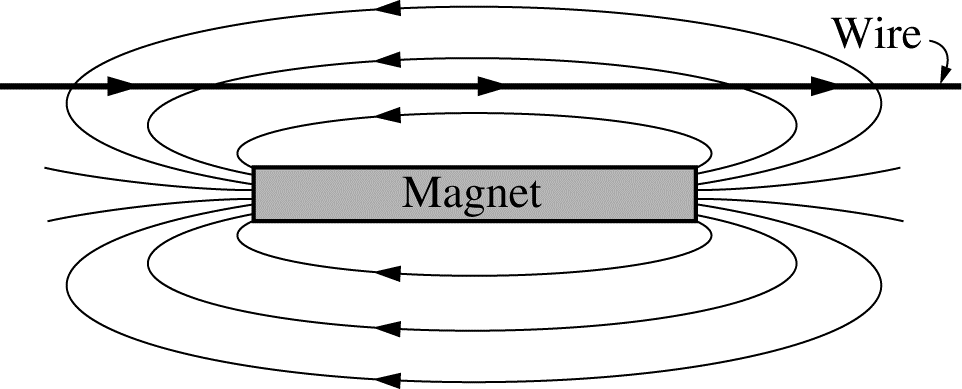
\includegraphics[scale=0.25]{images/img-013-027.png}
\end{center}

% Multiple Choice Question 29
\begin{questions}\setcounter{question}{28}\question
A wire is placed parallel to a bar magnet, as shown above, and carries current to the right. Several magnetic field lines outside the bar magnet are shown. Which of the following correctly describes the net magnetic force and torque on the wire?

\tabto{0.75cm}\underline{Net Force}
\tabto{7.00cm}\underline{Torque}

\begin{choices}
\choice Toward the top of the page    \tabto{6.25cm} Zero
\choice Toward the bottom of the page \tabto{6.25cm} Zero
\choice Toward the right              \tabto{6.25cm} Nonzero
\choice Zero                          \tabto{6.25cm} Zero
\choice Zero                          \tabto{6.25cm} Nonzero
\end{choices}\end{questions}

